\documentclass[../DefinizioneDiProdotto.tex]{subfiles}
\begin{document}

\section{Diagrammi di sequenza}

	In questa sezione vengono descritte e rappresentate tramite diagrammi di sequenza UML le sequenze di azioni ritenute più significative con lo scopo di facilitare la comprensione delle comunicazioni tra oggetti facenti parte dell'applicativo Android\g. Per quest'ultimo motivo i diagrammi di sequenza non rappresentano l'effettiva realtà ma una versione semplificata e che non rifletterà in tutto l'implementazione.
	
	\subsection{Avvio Service per il rilevamento beacon}
	
	
		Il diagramma in figura \ref{StartService} rappresenta l'avvio del service\g\ che si occupa del rilevamento dei beacon\g\, funzionalità focale dell'intero applicativo.
		
	La classe \verb|NavigationManagerPresenter| invoca il metodo \verb|startService()| su \verb|NavigationManagerImp|, all'interno del metodo viene istanziato un oggetto \verb|intent| di tipo \verb|Intent| necessario per creare effettivamente un bind service\g\, \verb|BeaconManagerAdapter|, attraverso la chiamata del metodo \verb|bindService()|,  passando come parametro \verb|intent|. 
	Nella fase di creazione del service\g\ \verb|BeaconManagerAdapter| viene chiamato il metodo \verb|onCreate()| nel quale viene creata un istanza della classe \verb|BeaconManager| offerta dalla libreria AltBeacon\g. Si effettuano inoltre diverse chiamate per il settaggio e la configurazione di \verb|beaconManager| che non sono rappresentate per mantenere il diagramma più leggibile. Una volta settato \verb|beaconManager| l'oggetto \verb|beaconManagerAdapter| si mette in ascolto di \verb|beaconManager| chiamando il metodo \verb|setMonitorNotifier| iniziando la fase di monitoring\g.
	
	A questo punto \verb|beaconManagerAdapter| è un listener di \verb|beaconManager| il quale una volta rilevata la region dei beacon in cui il device si trova scatena l'evento \verb|didEnterRegion()| notificando i propri listener, ossia l'oggetto di tipo \verb|beaconManagerAdapter|.
	
	Individuata la region tramite l'evento \verb|beaconManagerAdapter| effettua un controllo per capire se la region è riconosciuta dall'applicativo, se lo è \verb|beaconManagerAdapter| entra nella fase di ranging\g\ in cui saranno raccolti dettagliatamente i dati di tutti i beacon rilevati. \verb|beaconManagerAdapter| si mette in ascolto in modalità ranging di \verb|beaconManager| tramite la chiamata del metodo \verb|setRangeNotifier()|.
	
	A questo punto \verb|beaconManagerAdapter| riceve l'evento di rilevazione beacon attraverso il metodo \verb|didRangeBeaconsInRegion()| il quale restituisce una \verb|Collection| di \verb|Beacon| e la \verb|Region| di appartenenza.
	
	Per la gestione degli elementi all'interno della \verb|Collection| si rimanda al diagramma successivo.
	
		\begin{figure} [p]
			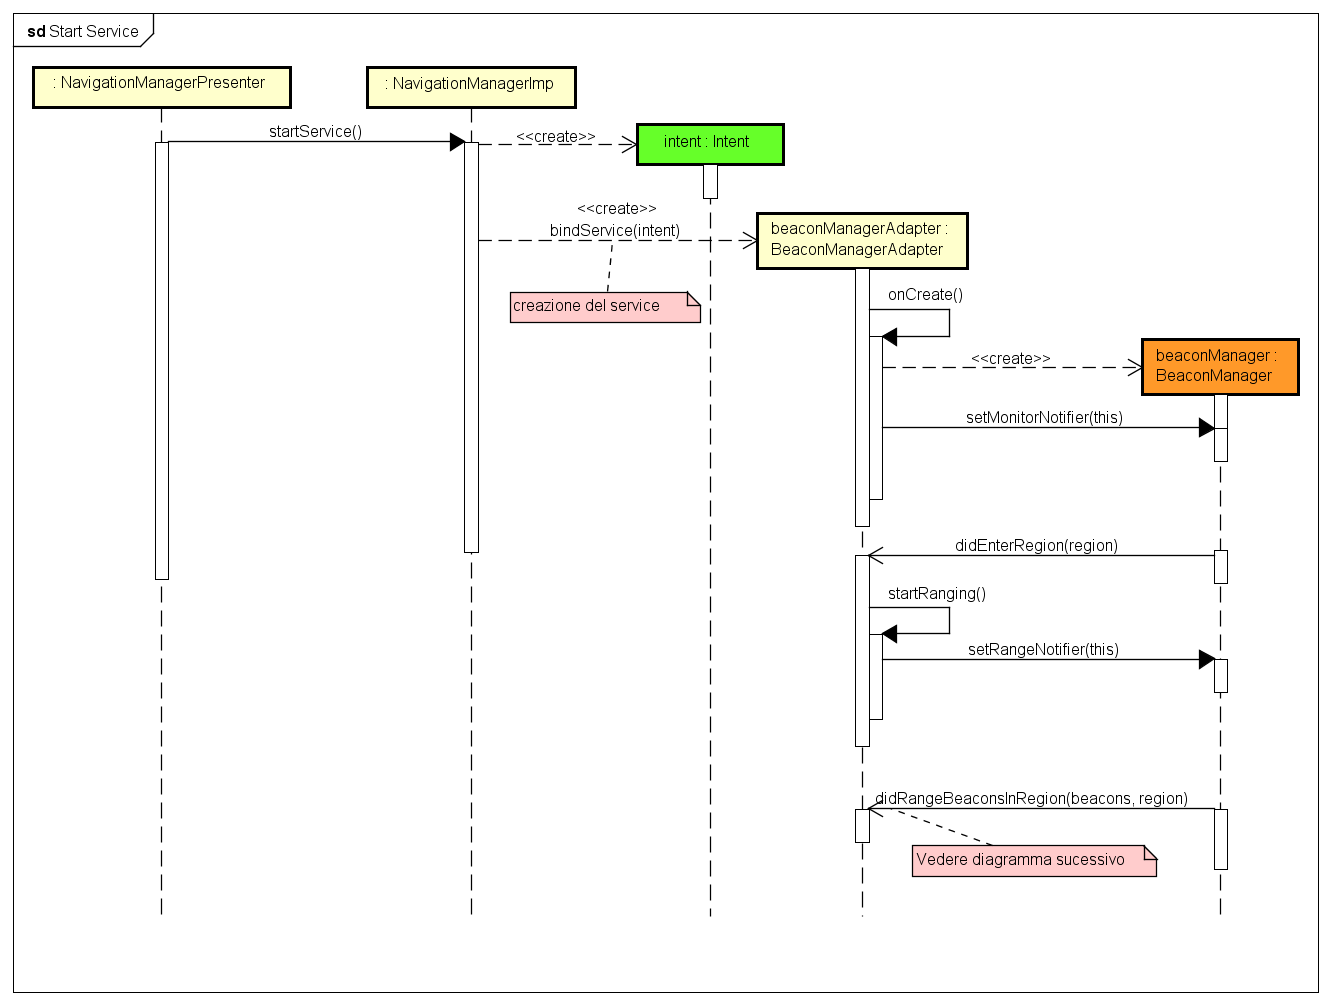
\includegraphics[width=\textwidth]{diagrams/StartService}
			\caption{Diagramma di sequenza - Avvio di un service\g\ per il rilevamento beacon}
			\label{StartService}
		\end{figure}
		

	\newpage		
	\subsection{Elaborazione beacon rilevati e comunicazione broadcast}
	
		Il diagramma in figura \ref{RangingBeacons} rappresenta l'interazione che avviene tra i componenti dell'applicativo allo scopo di rilevare dettagliatamente i dati trasmessi dai beacon circostanti al device.
		
L'oggetto di tipo \verb|BeaconManagerAdapter| è un service\g\ e implementa il listener di \verb|BeaconManager|: \verb|RangeNotifier| il quale scatenerà, dopo una scansione, l'evento  \verb|didRangBeaconsInRegion()| passando come parametri una \verb|Collection| di \verb|Beacon| rilevati e la \verb|Region| di appartenenza. 
	I parametri vengono elaborati da \verb|BeaconManagerAdapter| il quale dopo aver creato una \verb|PriorityQueue| costruisce un wrapper\g\ (\verb|MyBeacon|) di ogni \verb|Beacon| aggiungendolo alla \verb|PriorityQueue| tramite \verb|add()|.
	
	Una volta elaborati tutti i \verb|Beacon| ricevuti \verb|BeaconManagerAdapter| crea un messaggio \verb|Intent| in cui inserisce la \verb|PriorityQueue| tramite la chiamata del metodo \verb|putExtra()|. Costruisce l'oggetto \verb|LocalBroadcastManager| per utilizzarlo nella chiamata del metodo \verb|sendMessageBroadcast()| che si occuperà di inviare l'\verb|Intent| in altre parti dell'applicazione costruite appositamente per ricevere il messaggio ed elaborarlo, queste parti estenderanno la classe \verb|BroadcastReceiver| offerta dal SDK Android\g.

		\begin{figure} [p]
			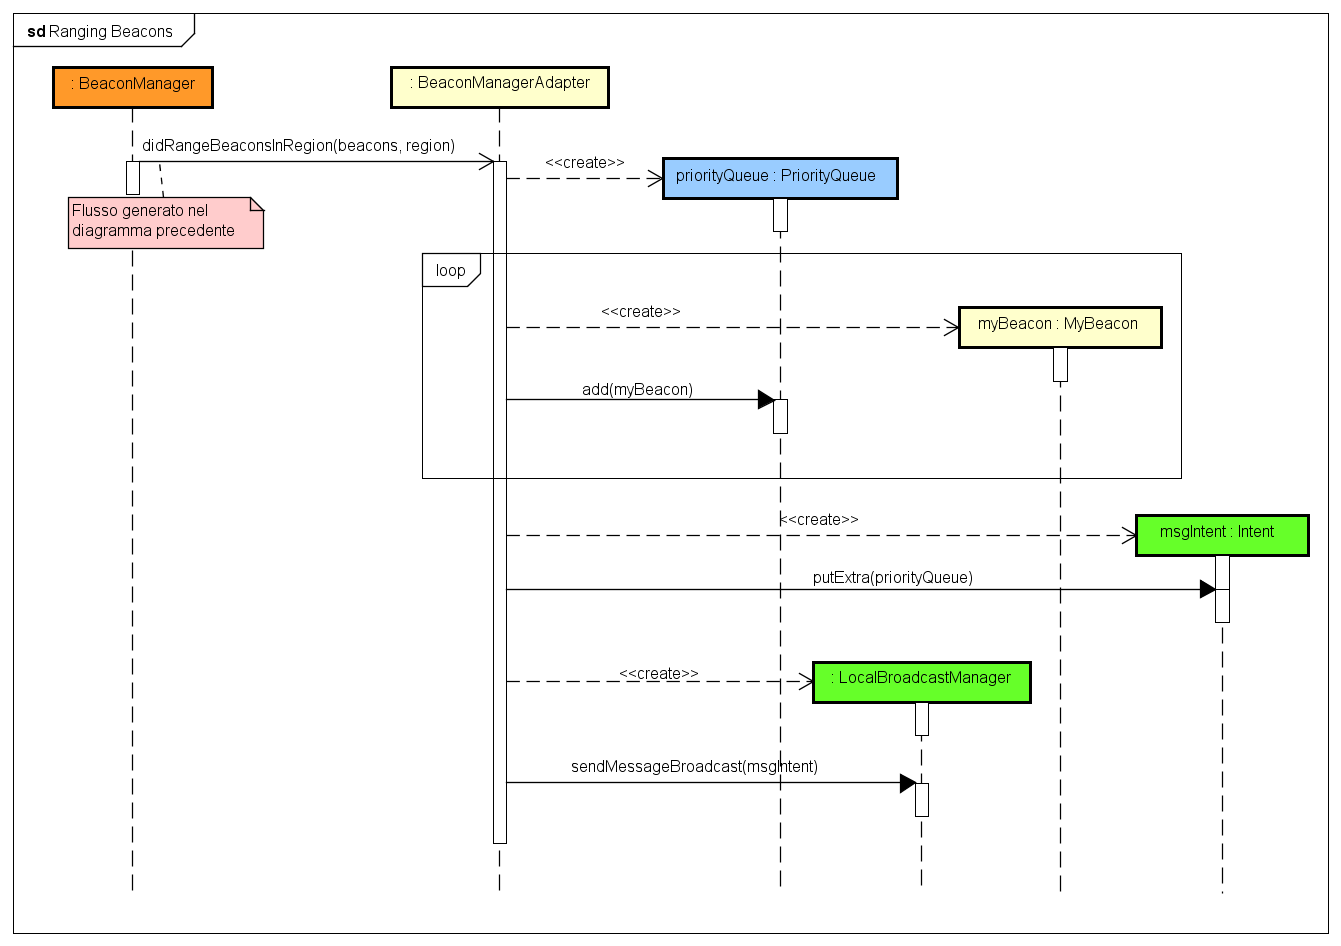
\includegraphics[width=\textwidth]{diagrams/RangingBeacons}
			\caption{Diagramma di sequenza - Elaborazione beacon rilevati e comunicazione broadcast}
			\label{RangingBeacons}
		\end{figure}
	
	
	\newpage
	\subsection{Avvio navigazione}
		
		Il diagramma in figura \ref{StartNavigation} rappresenta il flusso d'eventi generato nelle classi del model qualora si richiedesse l'avvio della navigazione. La richiesta parte da \verb|NavigationManagerPresenter| con la chiamata del metodo \verb|startNavigation()| sull'oggetto \verb|NavigatiorManagerImp| passando come parametri la destinazione identificata dall'oggetto di tipo \verb|PointOfInterest|. Il \verb|NavigatorManagerImp| si occupa quindi di impostare il grafo all'oggetto di tipo \verb|NavigatorImp| con il metodo \verb|setGraph()| dopodiché invoca il metodo \verb|calculatePath()| in cui è calcolato il percorso da seguire durante la navigazione attraverso l'oggetto \verb|DijkstraPathFinder| che restituisce una \verb|List| di \verb|EnrichedEdge| salvata in \verb|navigator| in un campo dati.
		A questo punto \verb|navigator| è pronto per restituire le informazioni (\verb|ProcessedInformation|) richieste dalla classe \verb|NavigationManagerImp|, quest'ultimo invoca il metodo \verb|toNextRegion()| passando come parametri la lista di beacon\g\ rilevati e ricevuti tramite l'oggetto \verb|BroadcastReceiver|.
		\verb|navigator| ricava dai beacon\g\ rilevati il beacon\g\ il cui segnale risulta essere il più potente (\verb|getMostPowerfulBEacon()|), quindi controlla che il beacon ritenuto più vicino all'utente appartiene alla region of interest (ROI\g) del percorso previsto, infine costruisce le \verb|ProcessedInformation| richieste grazie all'oggetto \verb|Edge| identificato come prossimo tratto di percorso da percorrere.
		Le \verb|ProcessedInformation| vengono quindi ritornate a \verb|NavigationManagerImp| che le restituisce a \verb|NavigationManagerImp| il quale le scompatterà e le restituirà alla view e quindi all'utente.
	
		\begin{figure} [h]
			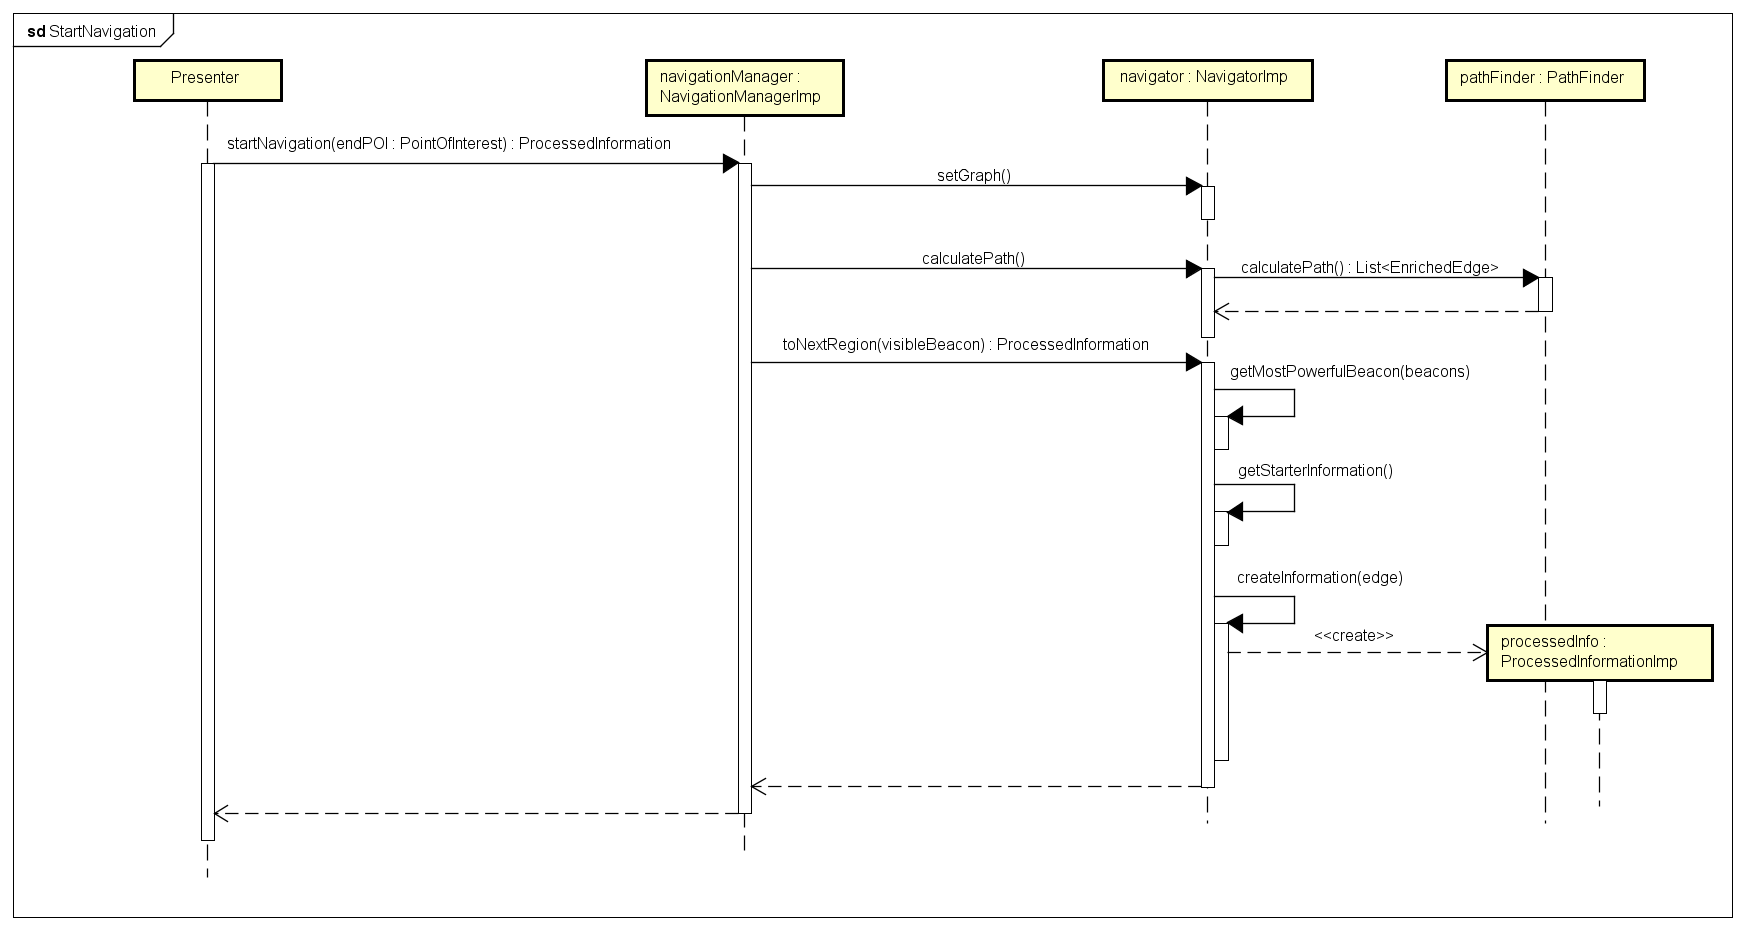
\includegraphics[width=\textwidth]{diagrams/StartNavigation}
			\caption{Diagramma di sequenza - Avvio navigazione}
			\label{StartNavigation}
		\end{figure}
		
		
\end{document}